% Created 2023-11-14 Tue 15:22
% Intended LaTeX compiler: pdflatex
\documentclass[11pt]{article}
\usepackage[utf8]{inputenc}
\usepackage[T1]{fontenc}
\usepackage{graphicx}
\usepackage{longtable}
\usepackage{wrapfig}
\usepackage{rotating}
\usepackage[normalem]{ulem}
\usepackage{amsmath}
\usepackage{amssymb}
\usepackage{capt-of}
\usepackage{hyperref}
\author{Hankertrix}
\date{\today}
\title{Carbohydrates Cheat Sheet}
\hypersetup{
 pdfauthor={Hankertrix},
 pdftitle={Carbohydrates Cheat Sheet},
 pdfkeywords={},
 pdfsubject={},
 pdfcreator={Emacs 29.1 (Org mode 9.6.6)}, 
 pdflang={English}}
\begin{document}

\maketitle
\setcounter{tocdepth}{2}
\tableofcontents \clearpage\newpage

\section{Definitions}
\label{sec:org90b1a52}

\subsection{Carbohydrates}
\label{sec:org49f8a54}
Carbohydrates are \textbf{polyhydroxyl aldehydes or ketones} with the general formula \(\boldsymbol{(CH_2O)_n}\).

\subsubsection{Functions of carbohydrates}
\label{sec:org73d24d9}
\begin{itemize}
\item \textbf{Cellular fuel}: Metabolism of sugars provide energy to run the cell and carbon atoms for biosynthesis.
\item \textbf{Cellular components}: Sugars are components of biomolecules and other cellular structures.
\end{itemize}

\subsection{Monosaccharides}
\label{sec:orgbcfea10}
Monosaccharides, or \textbf{simple sugars}, have from 3 to 7 carbon atoms, and one aldehyde or one ketone group. They cannot be broken down into simple sugars under mild conditions.

\subsection{Aldose}
\label{sec:org6b6a1ac}
Aldose is a sugar molecule that has an \textbf{aldehyde} group. The aldehyde group is always at the \textbf{end} of the carbon chain.

\subsection{Ketose}
\label{sec:orgc09416f}
Ketose is a sugar molecule that has a \textbf{ketone} group. The ketone group is always on the \textbf{second carbon} of the chain.

\subsection{Oligosaccharides}
\label{sec:orgc8955d0}
Oligosaccharides are made of 2 to 10 simple sugar residues.

\subsection{Polysaccharides}
\label{sec:org2ba8878}
Polysaccharides are polymers of monosaccharides. They contain \textbf{acetal and ketal} linkages, which are stable under physiological condition. \textbf{Enzymes} are needed to break the \textbf{glycosidic bonds} in polysaccharides.

\subsection{Disaccharides}
\label{sec:org3e83d08}
Disaccharides are also polymers of monosaccharides, but they are only made of 2 monosaccharides. They are two monosaccharides linked by a \textbf{glycosidic bond}, which is \(O-R\) bond, where the \(R\) group comes from the alcohol. The free substituted anomeric carbon is the \textbf{reducing} end, which means that \textbf{it itself gets oxidised}.
\begin{center}
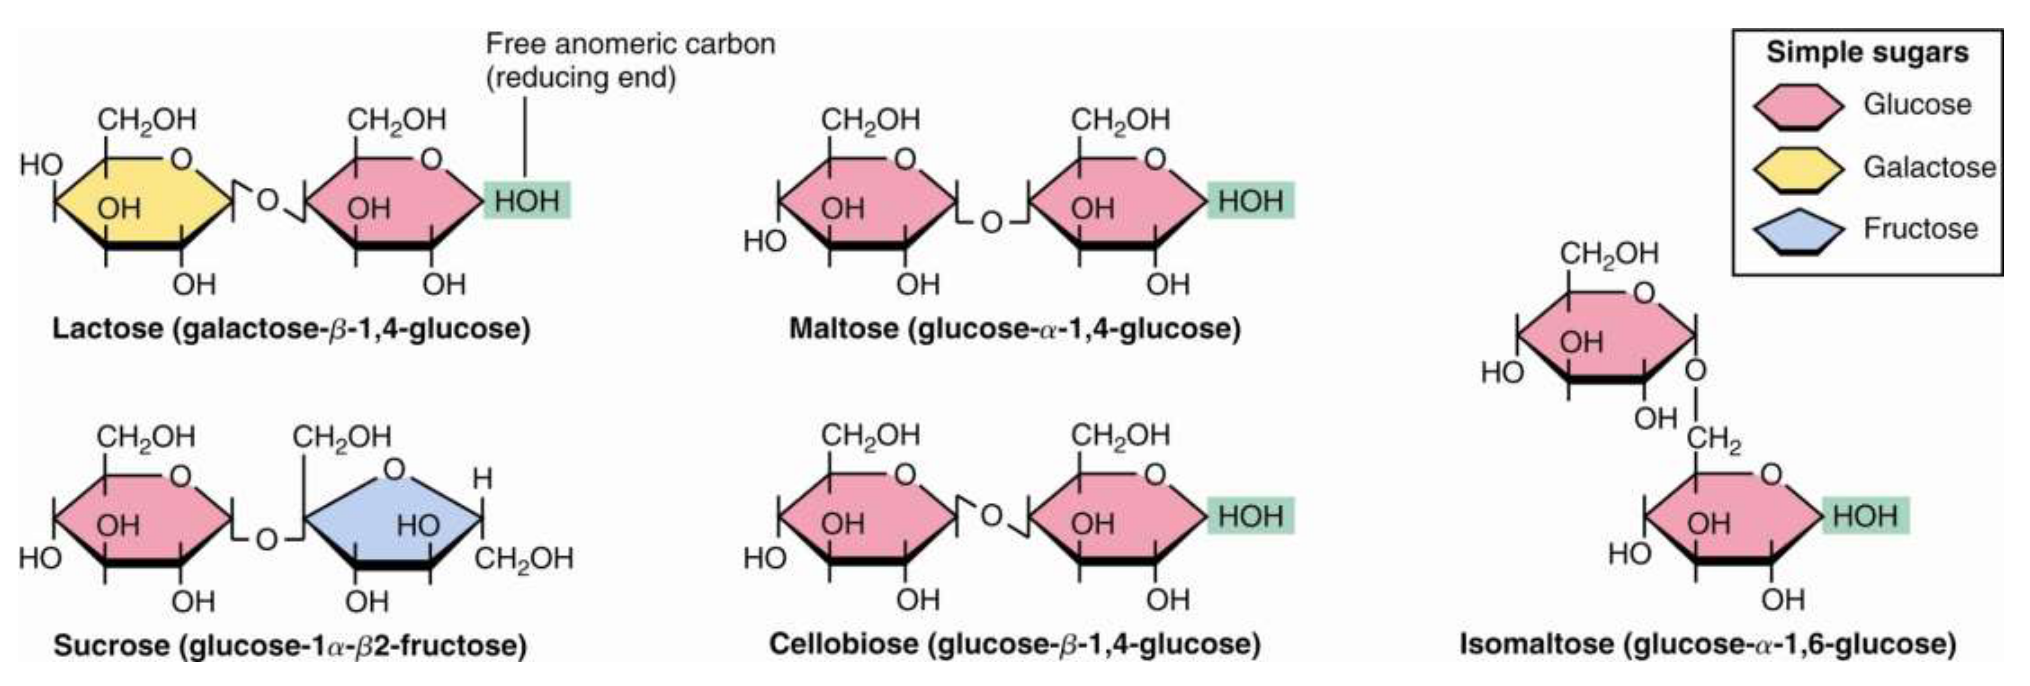
\includegraphics[width=.9\linewidth]{./images/disaccharides.png}
\end{center}

\subsection{Epimer}
\label{sec:orgf1a86dd}
Epimers are carbohydrates that differ in the location of the \(-OH\) group in \textbf{one} location.

\subsection{Tautomer}
\label{sec:org2f46d77}
Tautomers are structural isomers (constitutional isomers) of chemical compounds that readily interconvert, by relocating a proton (\(H^+\)) in a process called tautomerisation.
\begin{center}
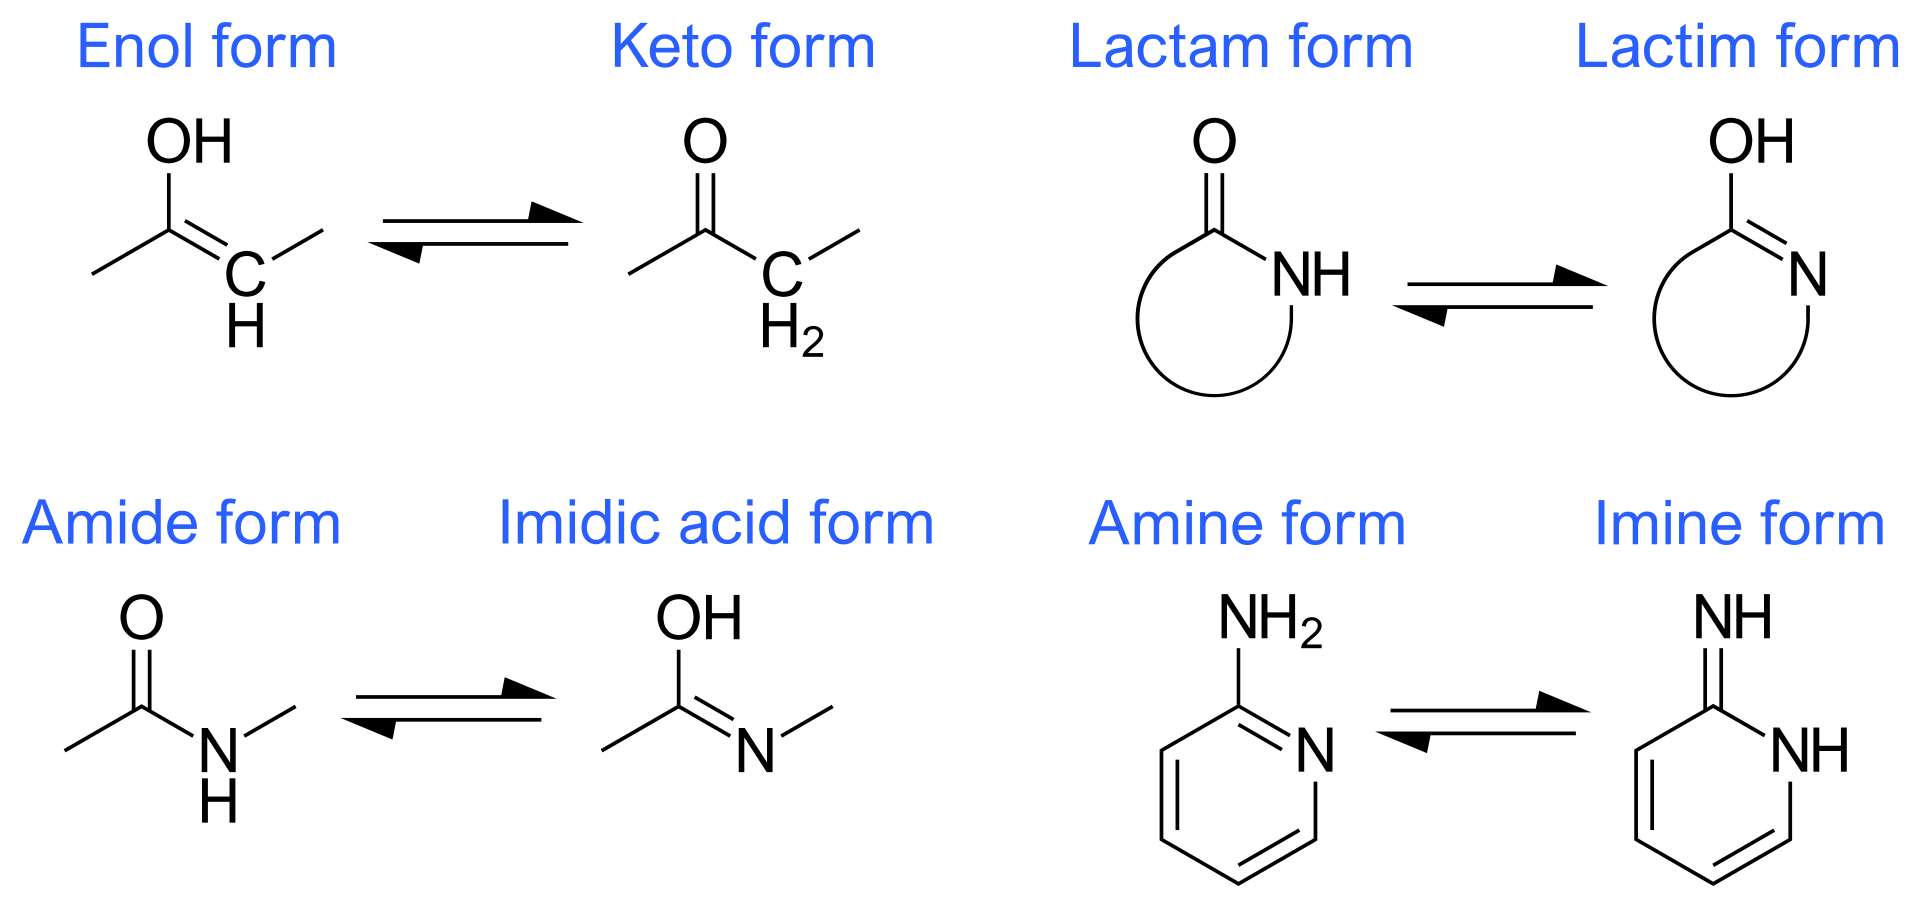
\includegraphics[width=.9\linewidth]{./images/tautomers.png}
\end{center}

\subsection{Mutarotation}
\label{sec:org03dfa30}
Mutarotation is the change in optical rotation of a chiral material due to the interconversion between the alpha (\(\alpha\)) anomeric form of a carbohydrate to its beta (\(\beta\)) anomeric form and vice versa.

\subsection{Carbonyl hydrate}
\label{sec:org3b9268a}
Carbonyl hydrate is the functional group shown below:

\begin{center}
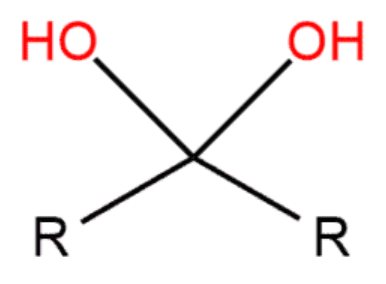
\includegraphics[scale=1.0]{./images/carbonyl-hydrate.png}
\end{center}

The mechanism is shown below:
\begin{center}
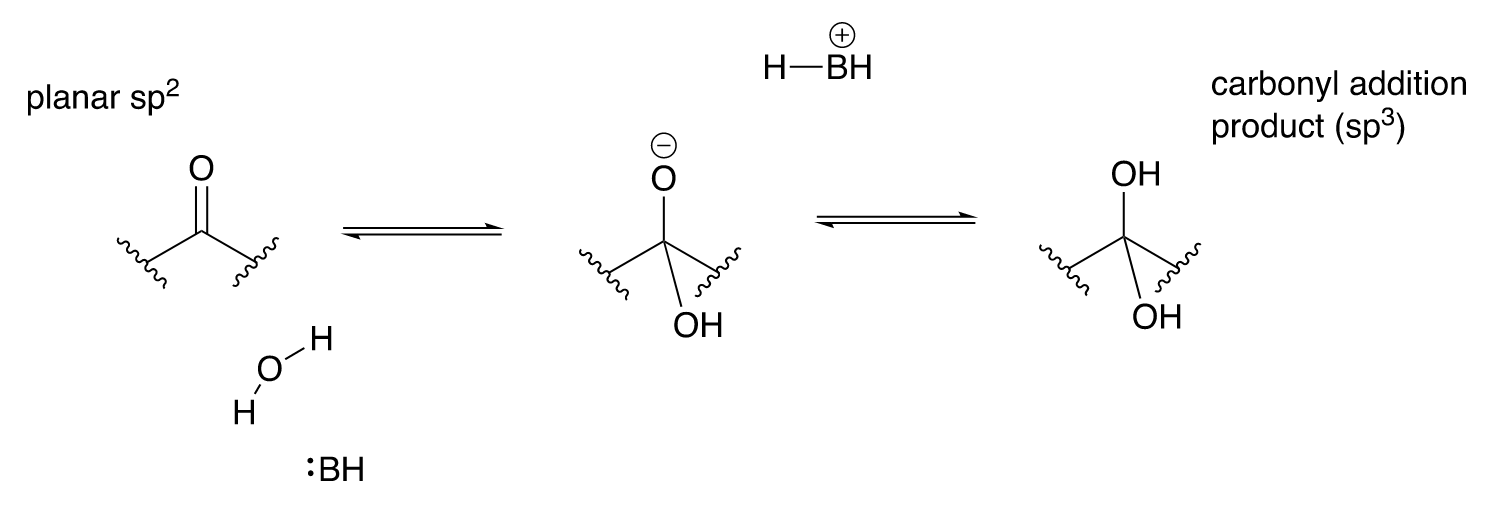
\includegraphics[width=.9\linewidth]{./images/carbonyl-hydrate-mechanism.png}
\end{center}

\newpage

\subsection{Hemiacetal}
\label{sec:orgaa57c4a}
Hemiacetal is the functional group shown below:

\begin{center}
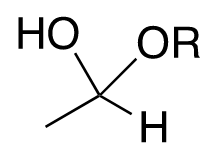
\includegraphics[scale=1.0]{./images/hemiacetal.png}
\end{center}

The mechanism is shown below:
\begin{center}
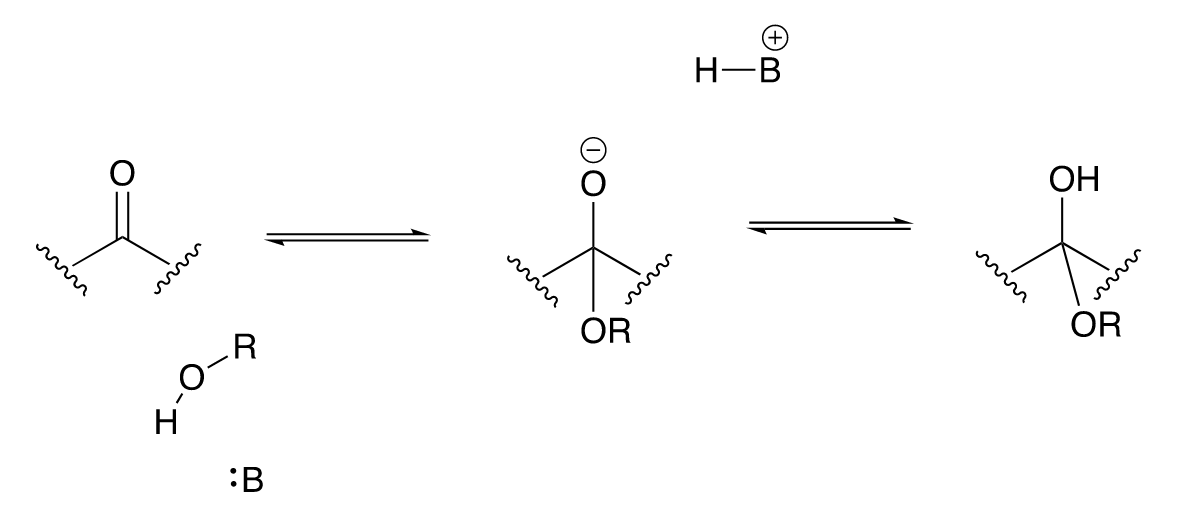
\includegraphics[width=.9\linewidth]{./images/hemiacetal-mechanism.png}
\end{center}

\textbf{Hemiketal} is just the hemiacetal functional group with its \textbf{hydrogen} replaced with a \(\boldsymbol{R}\) group. Both hemiacetal and hemiketal are \textbf{unstable} and are usually in rapid equilibrium with carbonyl and alcohol in aqueous solutions at physiological pH (pH 7.4).
\begin{center}
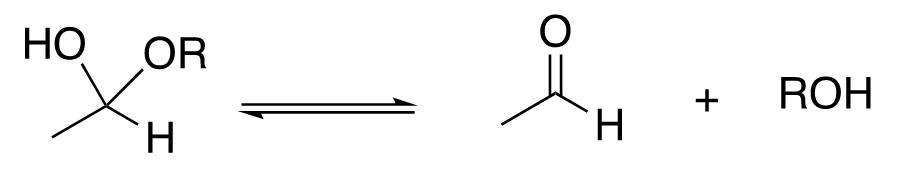
\includegraphics[width=.9\linewidth]{./images/hemiacetal-equilibria.png}
\end{center}

\newpage

\subsection{Acetal}
\label{sec:org5071566}
\textbf{Acetal} is the functional group shown below:

\begin{center}
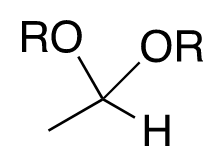
\includegraphics[scale=1.0]{./images/acetal.png}
\end{center}

\textbf{Ketal} is just the acetal functional group with its \textbf{hydrogen} replaced with a \(\boldsymbol{R}\) group. Both ketal and acetal are usually stable and are not in rapid equilibrium with carbonyl and alcohol in aqueous solutions at physiological pH (pH 7.4).

\subsection{Anomers}
\label{sec:orgc11eac7}
Anomers are cyclic monosaccharides that differ from each other in the configuration of the \(C\)-1 or \(C\)-2 carbon. For aldoses, it is the \(C\)-1 carbon, and for ketoses, it is the \(C\)-2 carbon. When the \(-OH\) group is \textbf{below} the carbon atom, it is called the \(\alpha\)-anomer, and when the \(-OH\) is \textbf{above} the carbon atom, it is called the \(\beta\)-anomer.

\subsection{Pyranose}
\label{sec:orgf4405fa}
Pyranose is a cyclic carbohydrate (sugar) with 6 members. The name comes from pyran, which is shown below:

\begin{center}
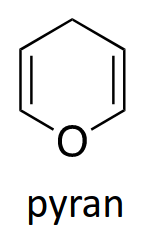
\includegraphics[scale=1.0]{./images/pyran.png}
\end{center}

\subsection{Furanose}
\label{sec:orgfe52e0a}
Furanose is a cyclic carbohydrate (sugar) with 5 members. The name comes from furan, which is shown below:

\begin{center}
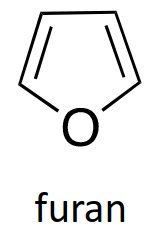
\includegraphics[scale=1.0]{./images/furan.png}
\end{center}

\subsection{Monosaccharide derivatives}
\label{sec:org9f04222}
Monosaccharide derivatives are molecules with functional groups that are derived from monosaccharides.

\subsubsection{Sugar alcohols}
\label{sec:org3961bc5}
Sugar alcohols are formed by mild reduction of sugars. Sugar alcohols such as sorbitol, mannitol, and xylitol sweeten many "sugarless" gums and candies.
\begin{center}
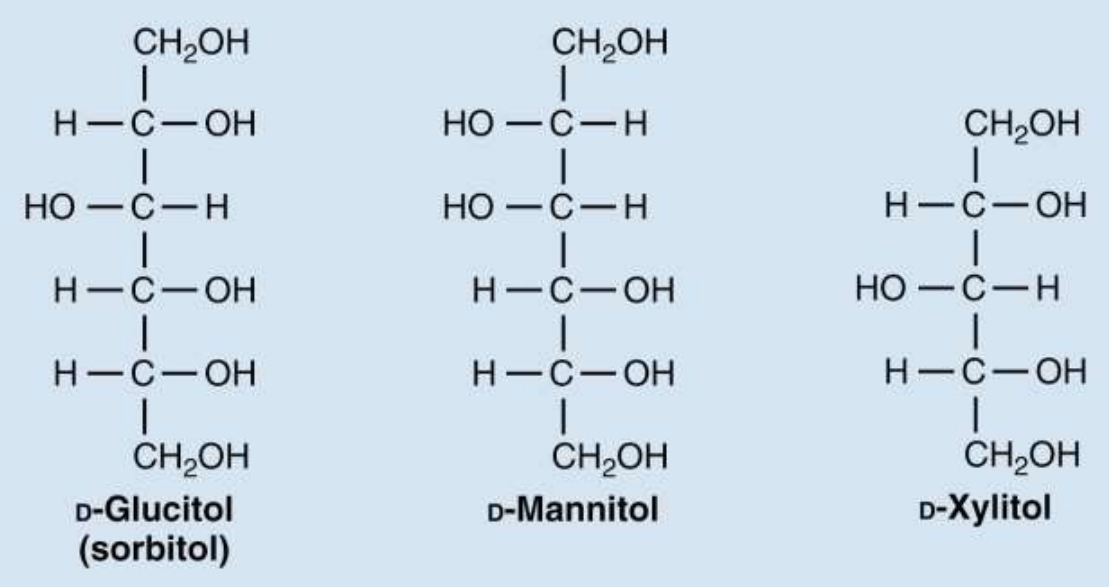
\includegraphics[width=.9\linewidth]{./images/sugar-alcohols.png}
\end{center}

\newpage

\subsubsection{Deoxy sugars}
\label{sec:orgef0e786}
Deoxy sugars are monosaccharides with one or more hydroxyl (\(-OH\)) groups replaced by hydrogens \(H\). 2-Deoxy-\(D\)-ribose is a constituent of DNA.
\begin{center}
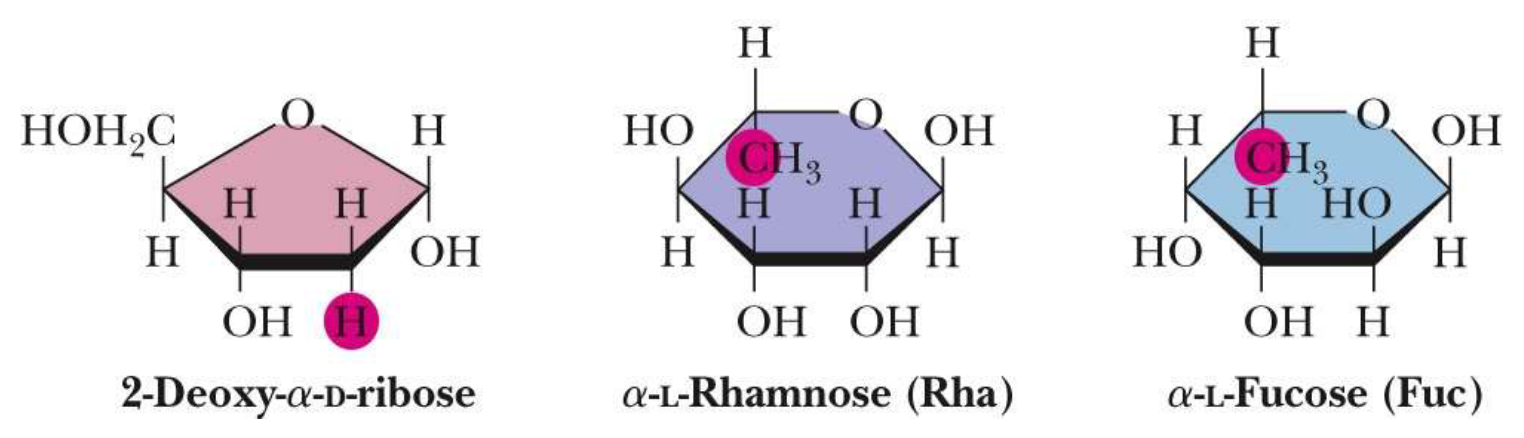
\includegraphics[width=.9\linewidth]{./images/deoxy-sugars.png}
\end{center}

\subsubsection{Sugar esters}
\label{sec:orgdb5064c}
Sugar esters are phosphate esters. The phosphate esters of glucose, fructose, and other monosaccharides are important metabolic intermediates. The ribose moiety of nucleotides such as ATP and GTP is phosphorylated at the 5' position.
\begin{center}
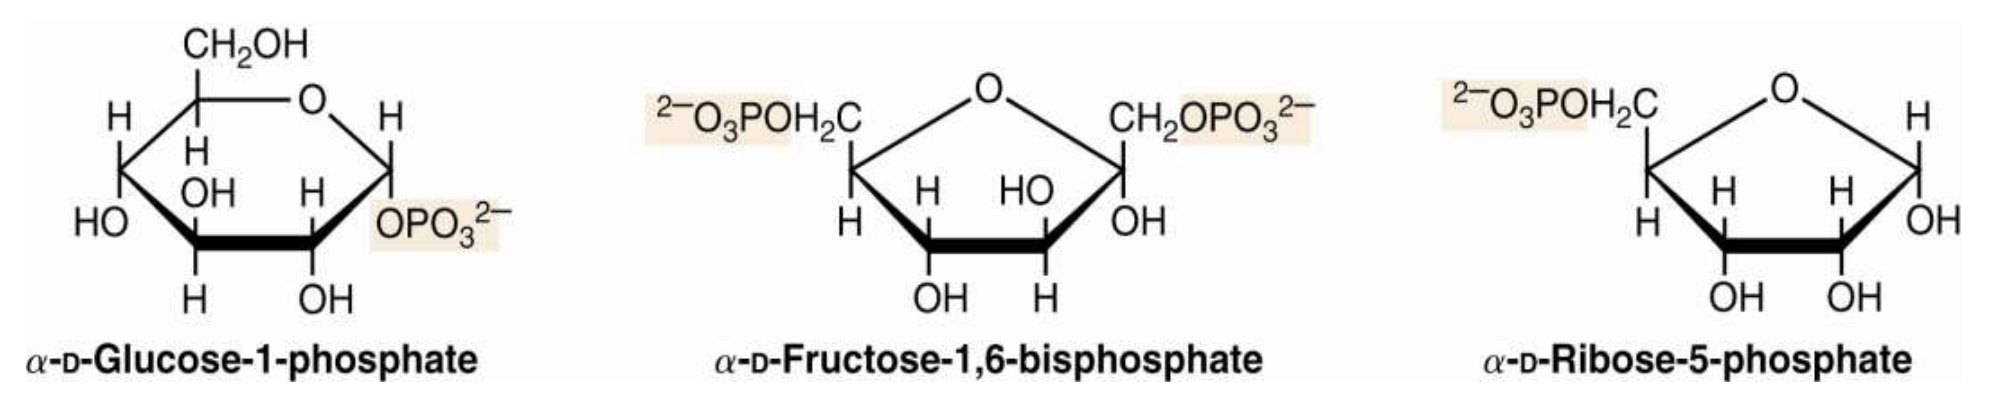
\includegraphics[width=.9\linewidth]{./images/sugar-esters.png}
\end{center}

\subsubsection{Amino sugars}
\label{sec:orgce037ce}
Amino sugars are sugars with an amino group at \(C\)-2. They are found in many oligosaccharides and polysaccharides.
\begin{center}
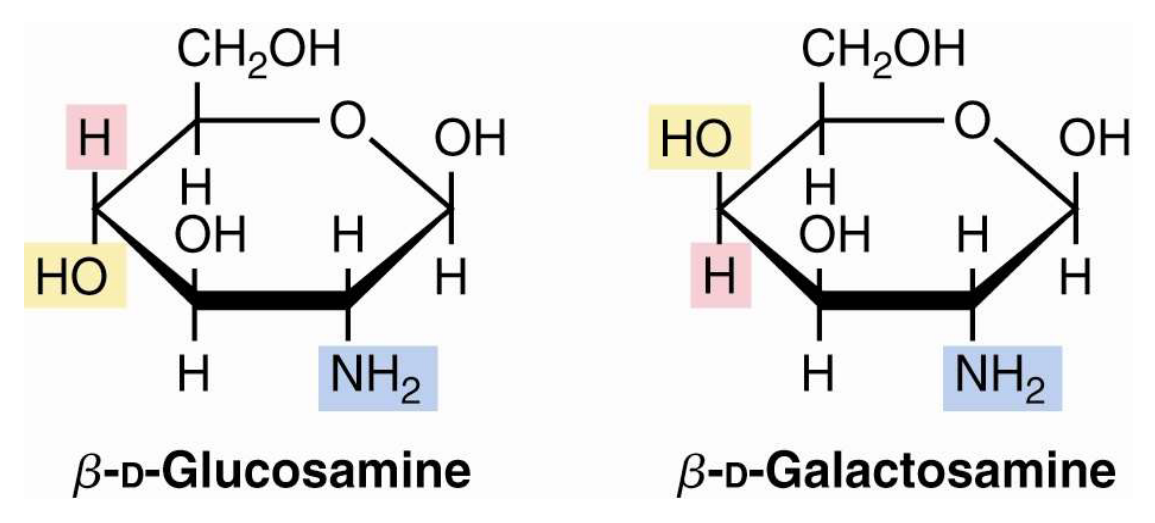
\includegraphics[width=.9\linewidth]{./images/amino-sugars.png}
\end{center}

\newpage

\subsubsection{Glycosides}
\label{sec:orge502a35}
Glycosides are the product of the dehydration reaction between monosaccharides and alcohols. This reaction retains the \(\alpha\)- or \(\beta\)-configuration at the \(C\)-1 carbon. The new bond is called a \textbf{glycosidic bond}.

\begin{center}
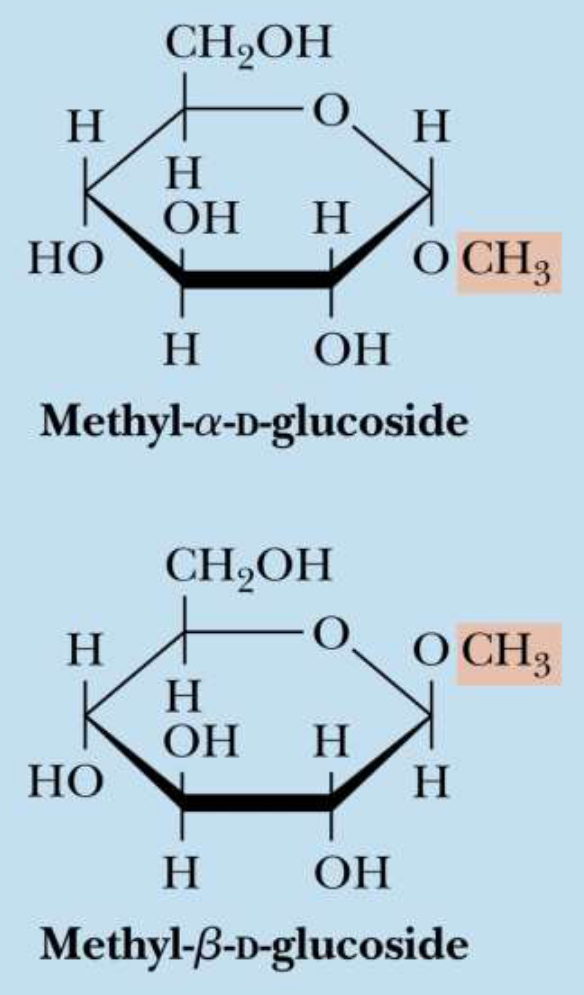
\includegraphics[scale=0.75]{./images/glycosides.png}
\end{center}


\section{Terminology of carbohydrates}
\label{sec:org2af075b}
The \emph{-ose} ending indicates a carbohydrate, and simple sugars are known by common names like \textbf{glucose}, \textbf{ribose}, and \textbf{fructose} rather than systematic names. The number of carbon atoms in an aldose or ketose is specified by the prefixes \emph{tri-}, \emph{tetra-}, \emph{pent-}, \emph{hex-}, or \emph{hept-}.


\section{Fischer projection forms}
\label{sec:org9409e7b}
\begin{itemize}
\item The stereochemistry at the chiral carbon \textbf{furthest away} (highest number) from the functional group (ketone or aldehyde) determines the \textbf{D or L} configuration.
\item \(-OH\) group on the right \(\rightarrow\) \textbf{D-configuration}
\item \(-OH\) group on the left \(\rightarrow\) \textbf{L-configuration}
\item Most naturally-occurring carbohydrates are in the D-configuration.
\end{itemize}

\subsection{Manipulation of Fischer projections}
\label{sec:org920a6a2}

\subsubsection{Fischer projections can only be rotated by \(180^{\circ}\)}
\label{sec:orgd2ea49a}
\begin{center}
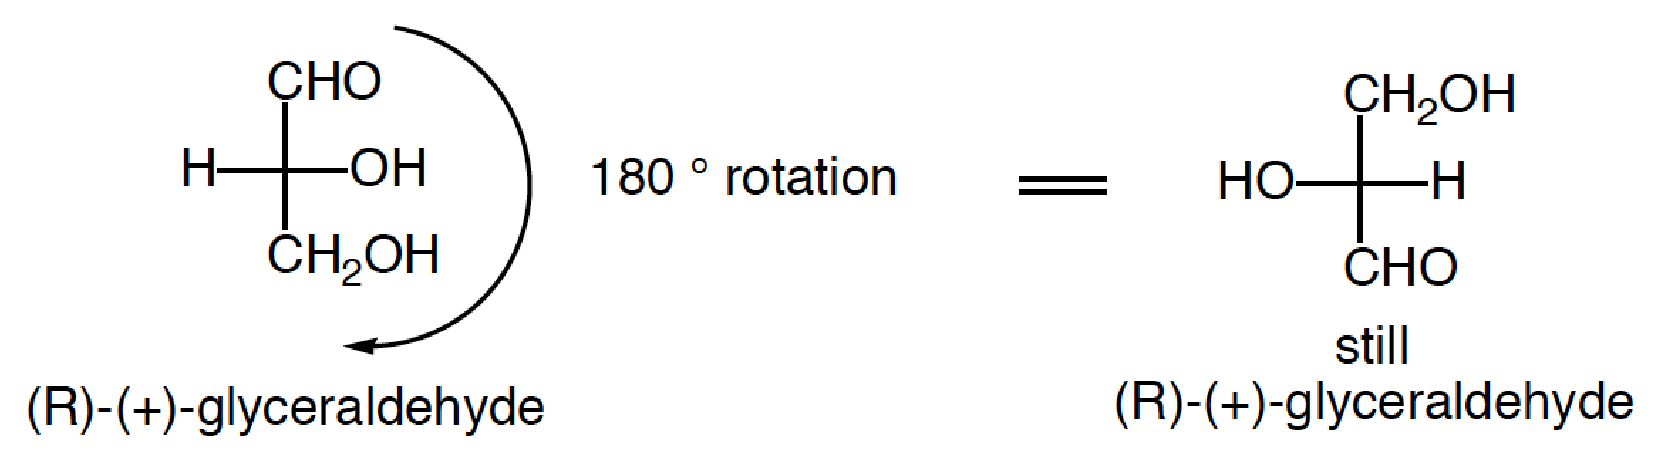
\includegraphics[width=.9\linewidth]{./images/180-rotation.png}
\end{center}

\subsubsection{Rotating \(90^{\circ}\) or \(270^{\circ}\) results in an enantiomer}
\label{sec:orgc246f3d}
\begin{center}
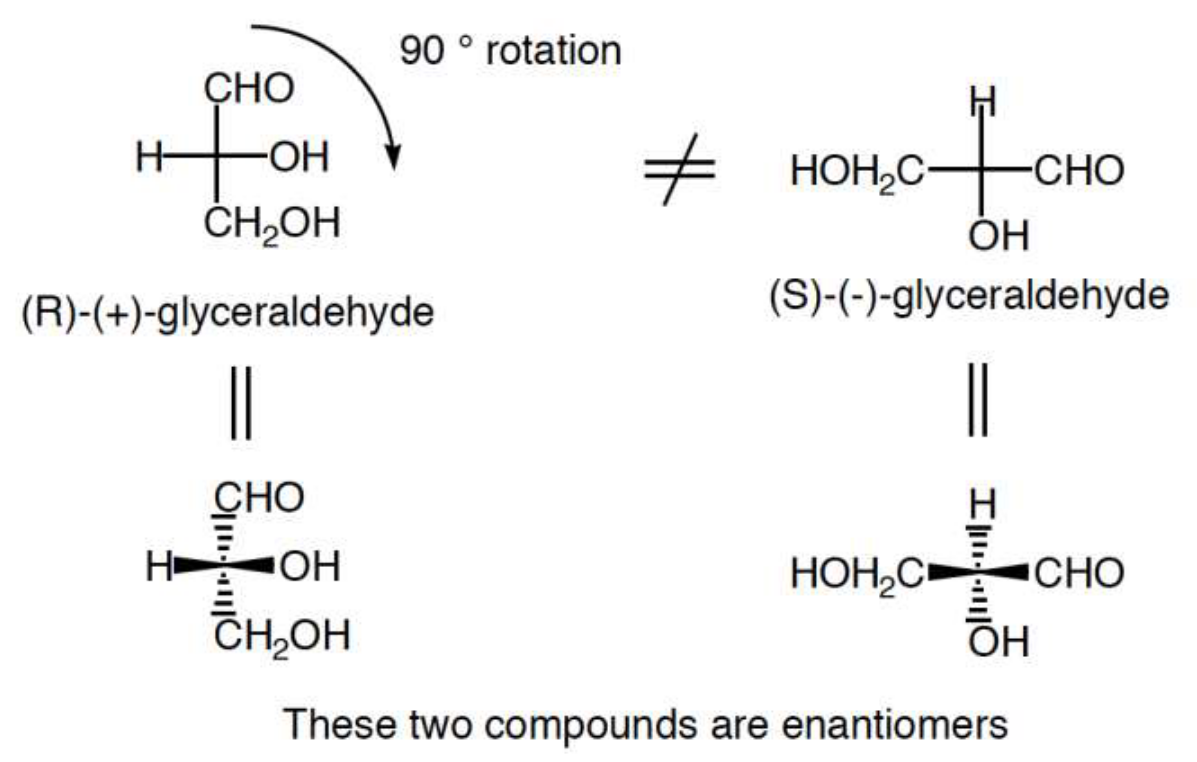
\includegraphics[width=.9\linewidth]{./images/90-rotation.png}
\end{center}

\subsubsection{If one group of the Fischer projection is held steady, the other groups can be rotated either clockwise or counterclockwise}
\label{sec:org4b27d69}
\begin{center}
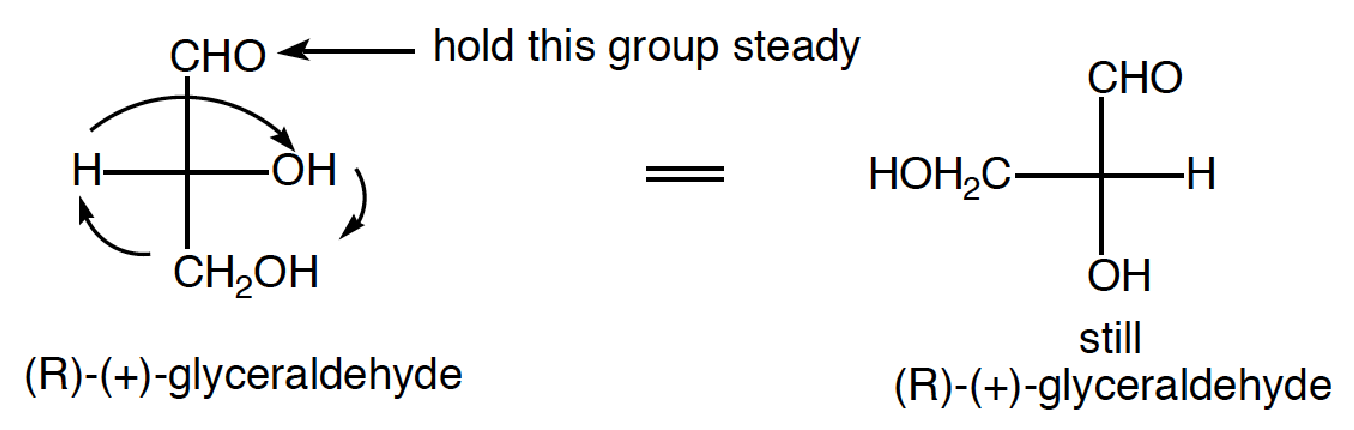
\includegraphics[width=.9\linewidth]{./images/three-group-rotation.png}
\end{center}


\section{Intramolecular carbonyl addition}
\label{sec:org422c767}
\begin{center}
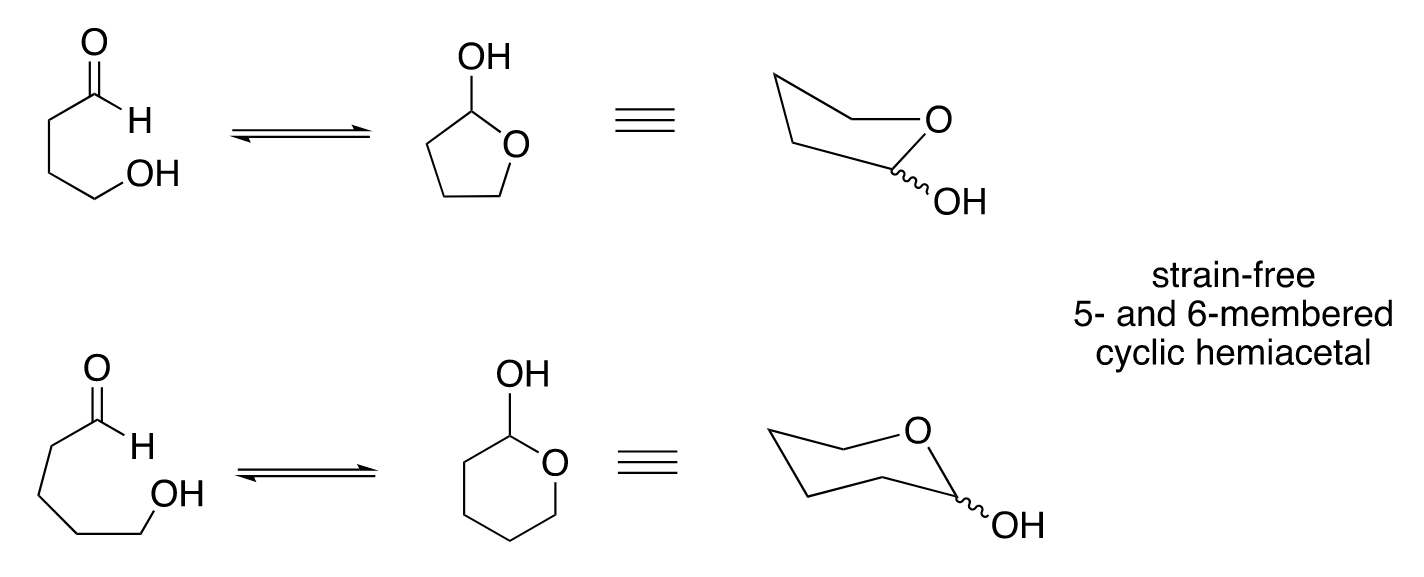
\includegraphics[width=.9\linewidth]{./images/intramolecular-carbonyl-addition.png}
\end{center}
\begin{center}
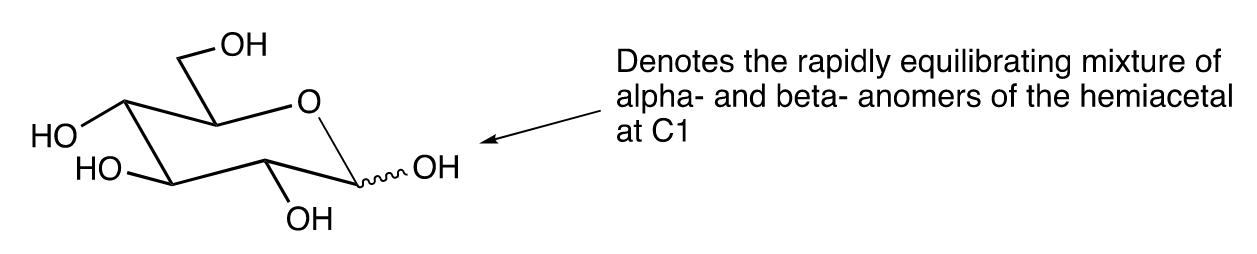
\includegraphics[width=.9\linewidth]{./images/rapidly-equilibriating-symbol-explanation.png}
\end{center}


\section{Haworth projection form}
\label{sec:orge39cd80}
\begin{center}
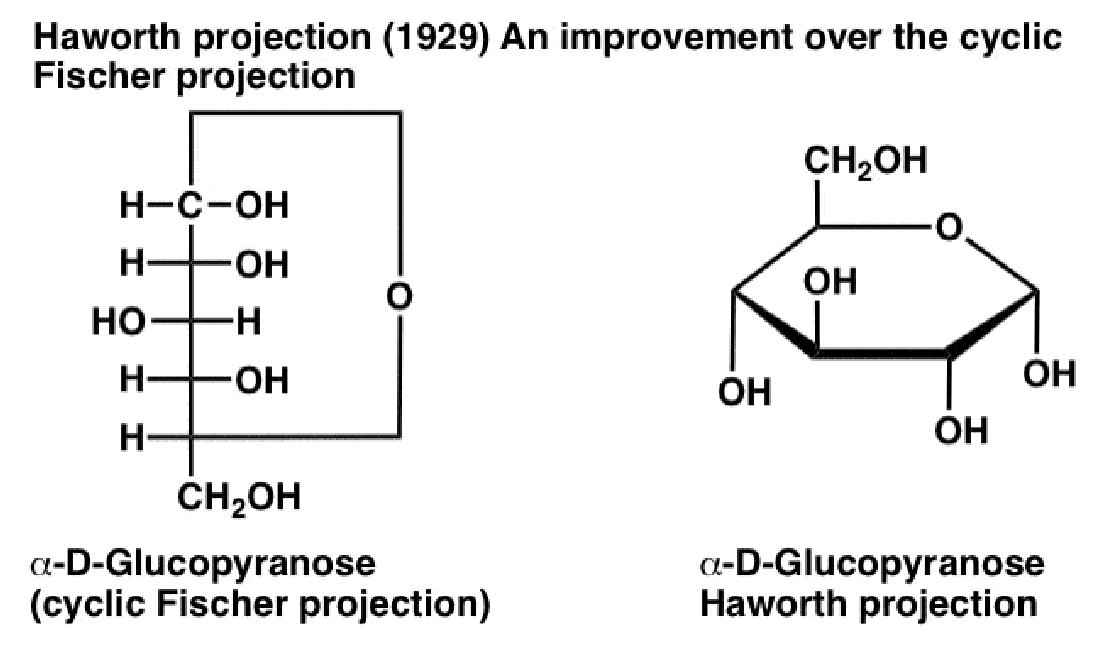
\includegraphics[width=.9\linewidth]{./images/haworth-projection.png}
\end{center}


\section{Formation of anomers}
\label{sec:org8c11f30}
\begin{center}
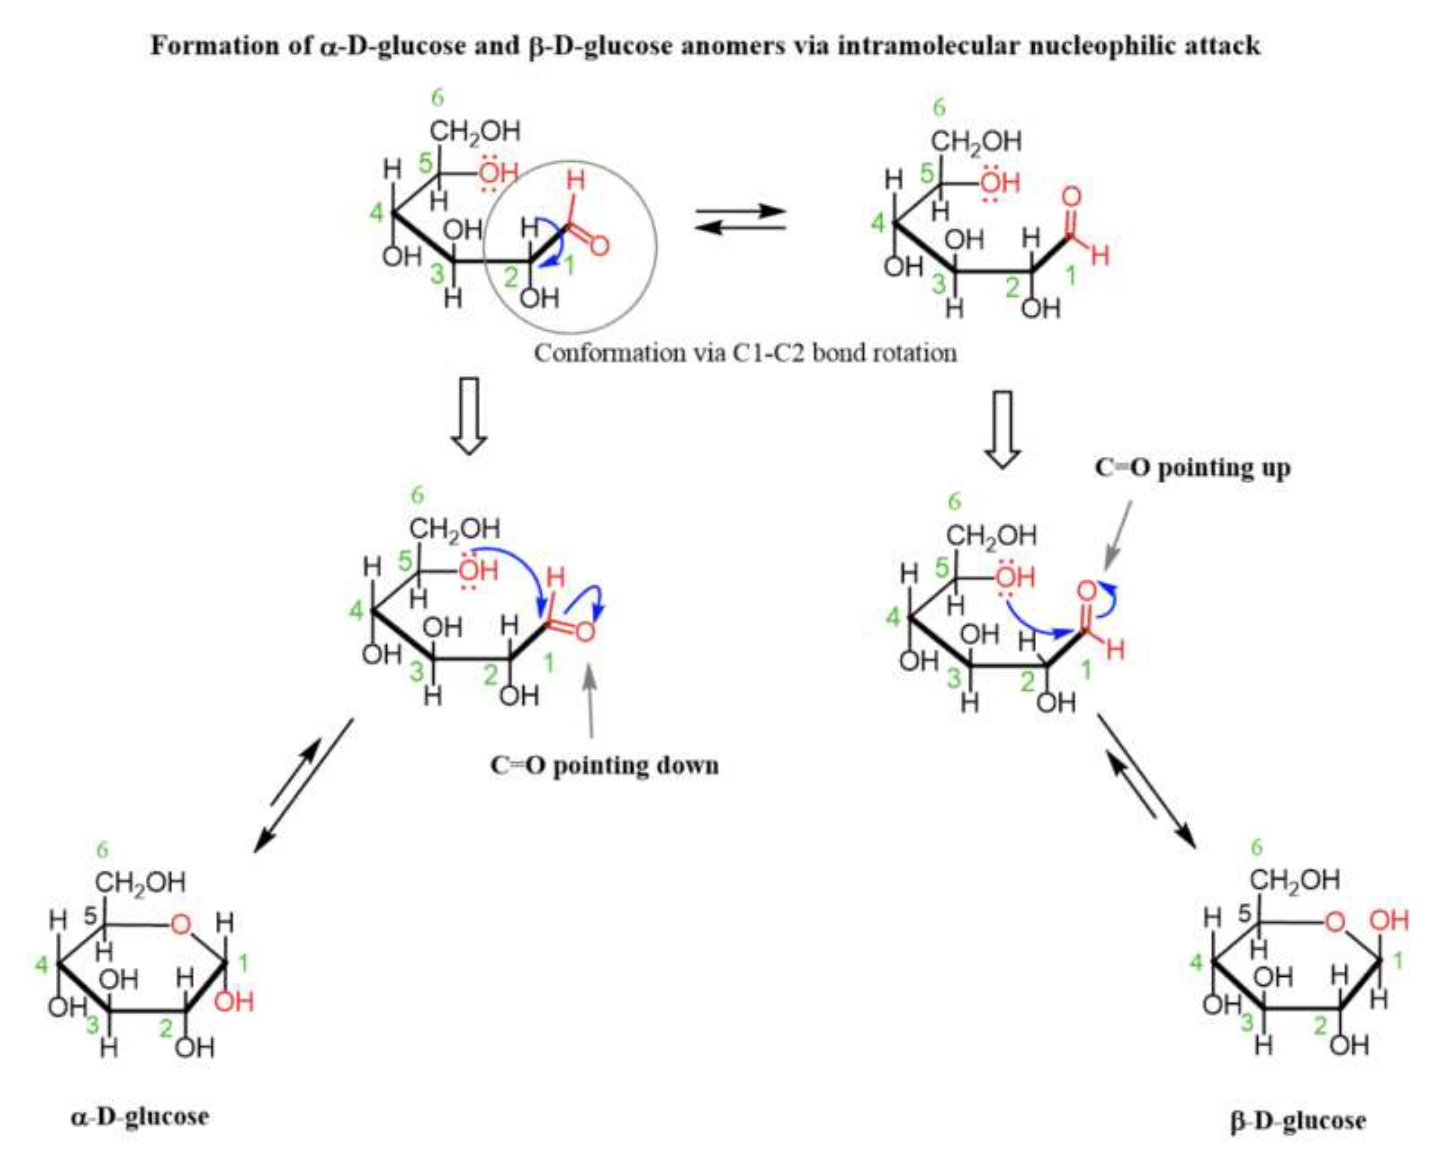
\includegraphics[width=.9\linewidth]{./images/formation-of-anomers.png}
\end{center}


\section{Common sugars in biological chemistry}
\label{sec:org23bb122}

\subsection{Pyranose}
\label{sec:org5441e89}

\subsubsection{D-glucose}
\label{sec:org3175960}

\begin{center}
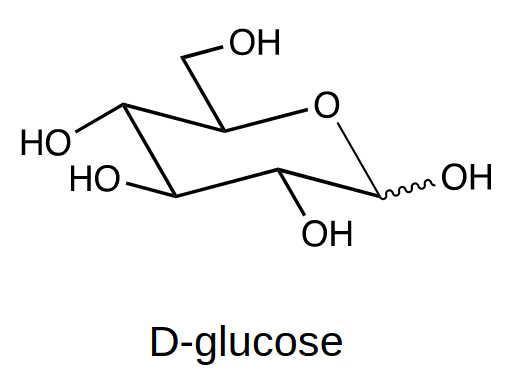
\includegraphics[scale=1.0]{./images/d-glucose.png}
\end{center}

\subsubsection{D-mannose}
\label{sec:orge9d2cae}

\begin{center}
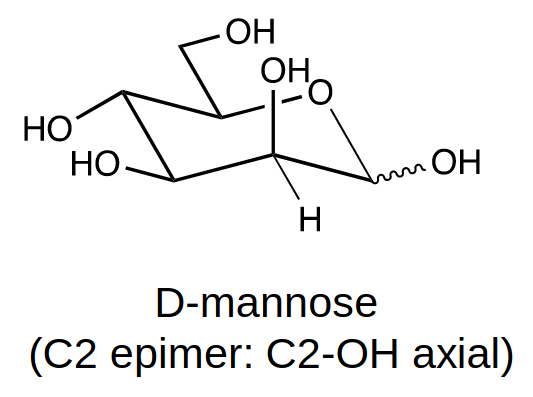
\includegraphics[scale=1.0]{./images/d-mannose.png}
\end{center}

\subsubsection{D-galactose}
\label{sec:org2f776f6}

\begin{center}
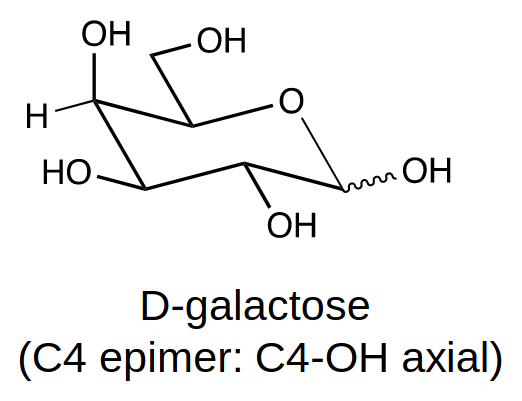
\includegraphics[scale=1.0]{./images/d-galactose.png}
\end{center}

\newpage

\subsection{Furanose}
\label{sec:org5d30b4e}

\subsubsection{Ribose}
\label{sec:orgbdd4eef}
\begin{center}
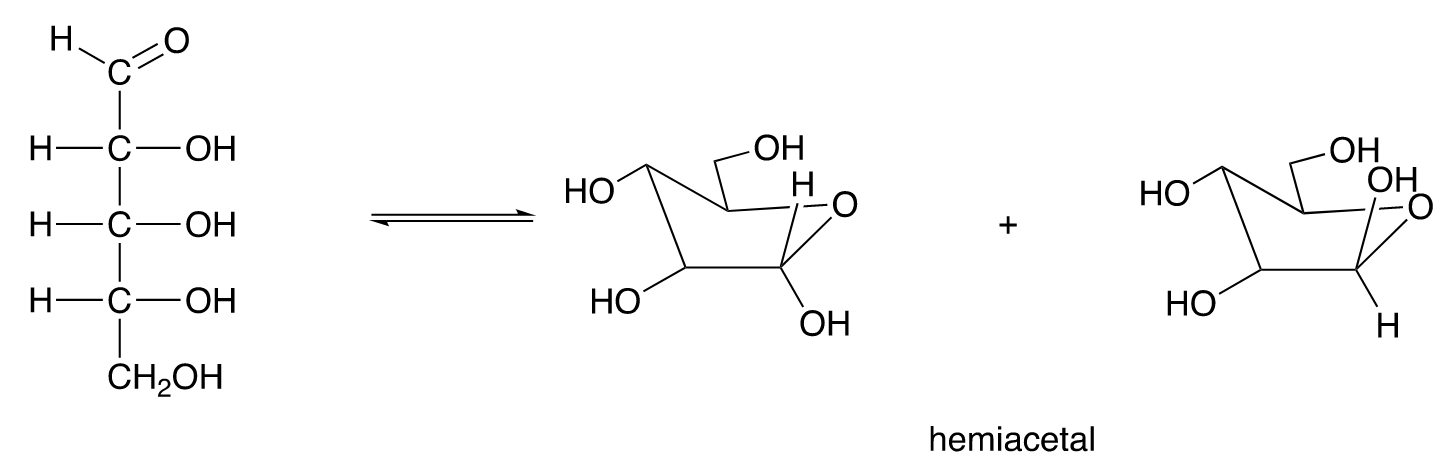
\includegraphics[width=.9\linewidth]{./images/ribose.png}
\end{center}

Ribose is used in adenosine triphosphate (ATP), which is shown below:
\begin{center}
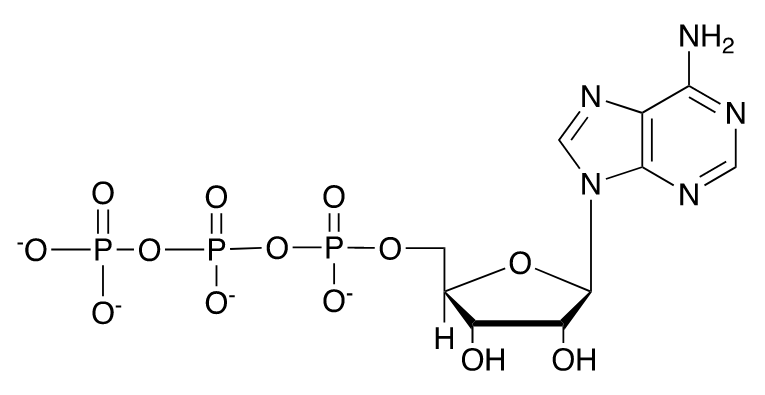
\includegraphics[width=.9\linewidth]{./images/atp.png}
\end{center}

\newpage

\subsection{Disaccharides}
\label{sec:org0f038a9}

\subsubsection{Lactose}
\label{sec:org9721c0d}
It's also known as galactosyl-beta-1,4-glucose.
\begin{center}
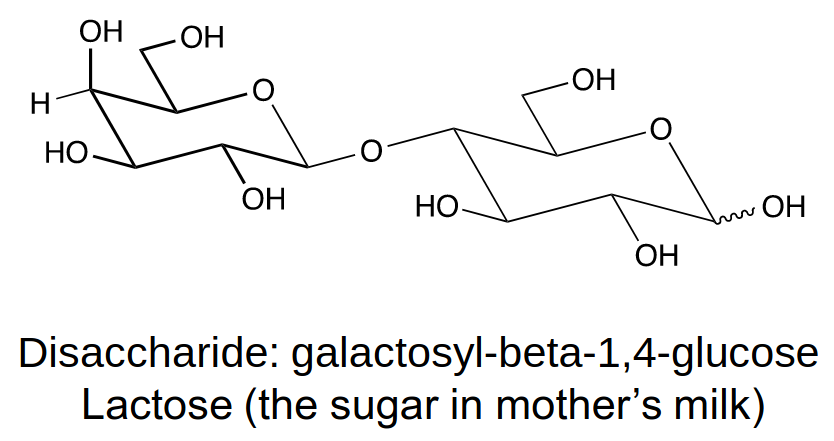
\includegraphics[width=.9\linewidth]{./images/lactose.png}
\end{center}

\subsubsection{Cellobiose}
\label{sec:org6ef0ebb}
It's also known as the glucosyl-beta-1,4-glucose.
\begin{center}
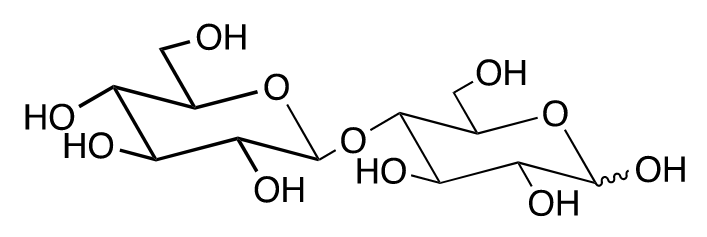
\includegraphics[width=.9\linewidth]{./images/cellobiose.png}
\end{center}

\newpage

\subsubsection{Maltose}
\label{sec:org08dbf38}
It's also known as the glucosyl-alpha-1,4-glucose.
\begin{center}
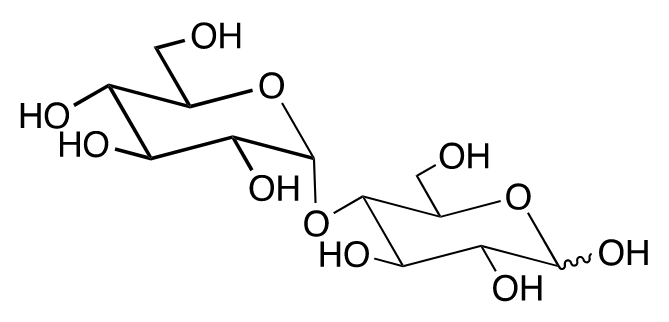
\includegraphics[width=.9\linewidth]{./images/maltose.png}
\end{center}

\subsection{Polysaccharides}
\label{sec:org340842b}

\subsubsection{Cellulose}
\label{sec:org959e3bd}
It is made up of poly-beta-1,4-glucosyl units and is used as a structural polymer in plants.
\begin{center}
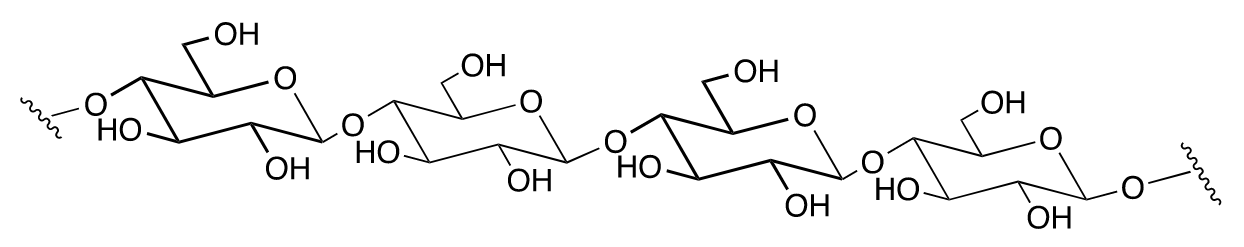
\includegraphics[width=.9\linewidth]{./images/cellulose.png}
\end{center}

\newpage

\subsubsection{Starch or glycogen}
\label{sec:org76cdae1}
It is made up of poly-alpha-1,4-glucosyl units and is used as an energy storage polymer in plants and animals.
\begin{center}
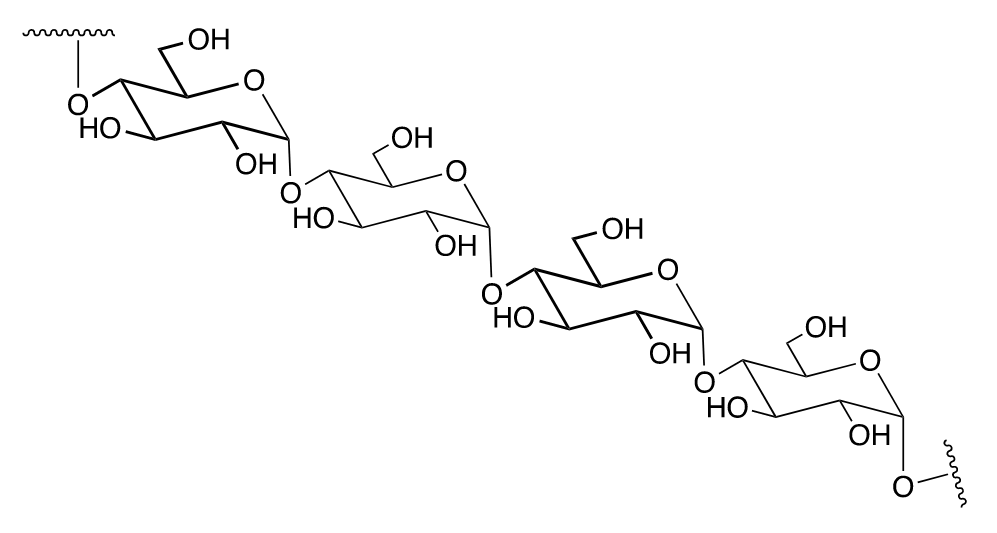
\includegraphics[width=.9\linewidth]{./images/starch.png}
\end{center}
\end{document}